\documentclass[a4paper, 11pt]{article}

% -- Coments
\usepackage{verbatim}

% ----- Fonts -----
% -- Fuente --
% \usepackage{fontspec}
% \setmonofont{JetBrainsMono Nerd Font}  

% -- Color --
\usepackage{xcolor}
%\definecolor{azul}{RGB}{00,33,99}
\definecolor{azul}{RGB}{35,72,180}

% -- Page Margin --
\usepackage[margin=1in]{geometry}

% -- Espaciados --
\newcommand{\Pspace}{0.5cm}
\newcommand{\Aspace}{0.2cm}

% -- Columnas --
\usepackage{multicol}

% -- Imagenes --
\usepackage{graphicx}
\usepackage{float}

% -- Matemáticas --
\usepackage{amsmath, amssymb}

% -- Gráficas --
\usepackage{pgfplots}
\pgfplotsset{compat=1.18}

\usepackage{svg}

% -- Código --
\usepackage{listings}
\usepackage{xcolor}

\definecolor{bg}{RGB}{246, 248, 250}
\definecolor{keyword}{RGB}{207, 34, 46}     % rojo
\definecolor{string}{RGB}{10, 106, 84}      % verde oscuro
\definecolor{comment}{RGB}{110, 119, 129}   % gris
\definecolor{builtin}{RGB}{111, 66, 193}    % morado
\definecolor{linenums}{RGB}{180, 185, 190}

\lstset{
    language=Python,
    basicstyle=\ttfamily\small,
    backgroundcolor=\color{bg},
    keywordstyle=\color{keyword}\bfseries,
    commentstyle=\color{comment}\itshape,
    stringstyle=\color{string},
    numberstyle=\tiny\color{linenums},
    numbers=left,
    breaklines=true,
    frame=single,
    rulecolor=\color{linenums}
}

\usepackage{minted}
\setminted{
    fontsize=\small,
    breaklines=true,               % Ajusta el código al ancho de página
    frame=lines,                   % Añade líneas arriba y abajo
    framesep=2mm,
    baselinestretch=1.2,
    bgcolor=lightgray!10           % Color de fondo muy suave
}

\begin{comment}
-- Formato de pregunta simple
    % - Problema n
    \vspace{\Pspace}
    \item Problema \par
        % Respuesta:
        \vspace{\Aspace} \par
        { \color{azul}  }


 -- Formato de pregunta multimple
        % - Problema 
        \vspace{\Pspace}
        \item  \par
             % Respuestas:
            \vspace{\Aspace} \par
            a) 
            \\ { \color{azul} }

            \vspace{\Aspace} \par
            b) 
            \\ { \color{azul} }


 -- Formato de imagen
\begin{figure}[!ht]
    \centering
    \includegraphics[width=0.5\textwidth]{}
\end{figure}


 -- Formato de tabla
\begin{tabular}{c|c}
    \textbf{A} & \textbf{B} \\
    \hline
    Texto & Texto \\
    Texto & Texto
\end{tabular} \\
\end{comment}


\title
{
    \textbf{Fluidos y Fenómenos Térmicos} \\
    Parcial 3 \\
    \Large{ Martha Anahí Iñiguez Beltrán }
}

\begin{document}

\maketitle

\begin{center}
    \begin{tabular}{r|l}
        \textbf{Expediente} & \textbf{Nombre} \\ \hline
        219208106 & Bórquez Guerrero Angel Fernando \\
    \end{tabular}
\end{center}

\rule{\linewidth}{0.3mm}

\vspace{0.3cm}
\Large{ \textbf{ Parte 1 } }
\begin{itemize}
    \item Definir la función de Mxwell-Boltzmann
    \item Generar dos distribuciones a distintas temperaturas
    \item Graficarlas correctamente
\end{itemize}
La masa a utilizar es de $m = 4.65E-26 Kg$ (masa de la molécula de nitrógeno). \\
La función de distribución de Maxwell-Boltzmann es:
\vspace{0.3cm}
\[ f(v) = 4 \pi \left( \frac{m}{2 \pi k T} \right)^{3/2} v^{2} e^{- \frac{mv^2}{2 k T}} \]

\vspace{0.3cm}
\includesvg[height=0.8em]{./img/python_logo.svg} Python - Función de distribución
\begin{lstlisting}
import numpy as np
import matplotlib.pyplot as plt
from scipy.constants import Boltzmann

# Constantes
k = Boltzmann   # Constante de Boltzmann
m = 4.65e-26    # Masa de una molécula

# Función de distribución
def maxwell_boltzmann(v, T):
    return (4 * np.pi * 
           (m / (2 * np.pi * k * T))**(3/2) * 
           v**2 * np.exp(- (m * v**2) / (2 * k * T)))
\end{lstlisting}

\newpage
\includesvg[height=0.8em]{./img/python_logo.svg} Python - Variables
\begin{lstlisting}
# Rango de velocidades
v = np.linspace(0, 1600, 1000)

# Temperaturas
T1 = 300
T2 = 500

# Distribuciones
f1 = maxwell_boltzmann(v, T1)
f2 = maxwell_boltzmann(v, T2)
\end{lstlisting}

\vspace{0.3cm}
\includesvg[height=0.8em]{./img/python_logo.svg} Python - Gráfica
\begin{lstlisting}
plt.figure(figsize=(10, 6))
plt.plot(v, f1, label=f"T = {T1} K")
plt.plot(v, f2, label=f"T = {T2} K")

plt.xlabel("Velocidad (m/s)")
plt.ylabel("Probabilidades")
plt.title("Distribución de Maxwell-Boltzmann")
plt.legend()
plt.grid()
plt.show()
\end{lstlisting}

\begin{figure}[!ht]
    \centering
    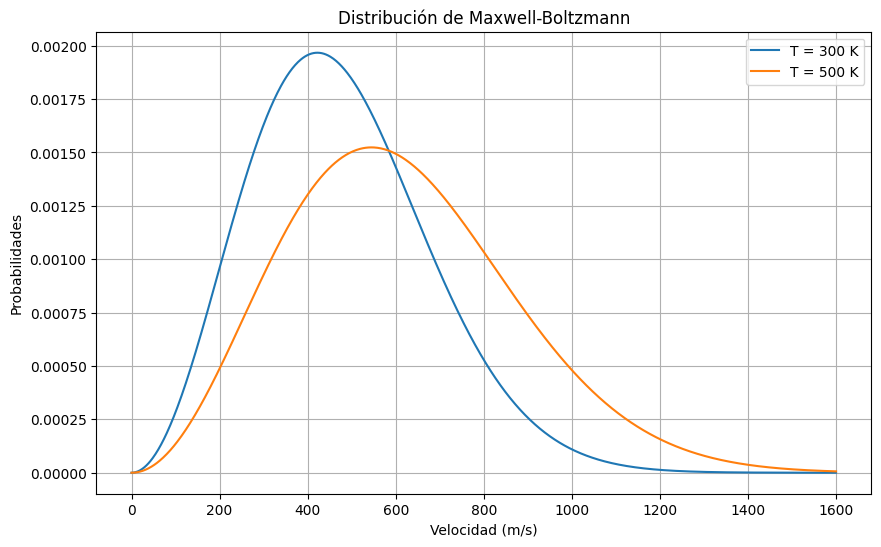
\includegraphics[width=0.9\textwidth]{./img/parte_1.png}
\end{figure}



\newpage
\Large{ \textbf{ Parte 2 } } \\
Agrega al código una región sombreada para representar las moléculas con velocidad mayor a:
\[ v_{escape} = 1000 m/s \]

\vspace{0.3cm}
\includesvg[height=0.8em]{./img/python_logo.svg} Python - Gráfica con representación de moléculas mayor a 1000 m/s
\begin{lstlisting}
v_escape = 1000

plt.figure(figsize=(10, 6))
plt.plot(v, f1, label=f"T = {T1} K")
plt.plot(v, f2, label=f"T = {T2} K")
plt.fill_between(v, f1, where=(v > v_escape), alpha=0.3)
plt.fill_between(v, f2, where=(v > v_escape), alpha=0.3)

plt.xlabel("Velocidad (m/s)")
plt.ylabel("Probabilidades")
plt.title("Moléculas con suficiente energía para escapar")
plt.legend()
plt.grid()
plt.show()
\end{lstlisting}

\begin{figure}[!ht]
    \centering
    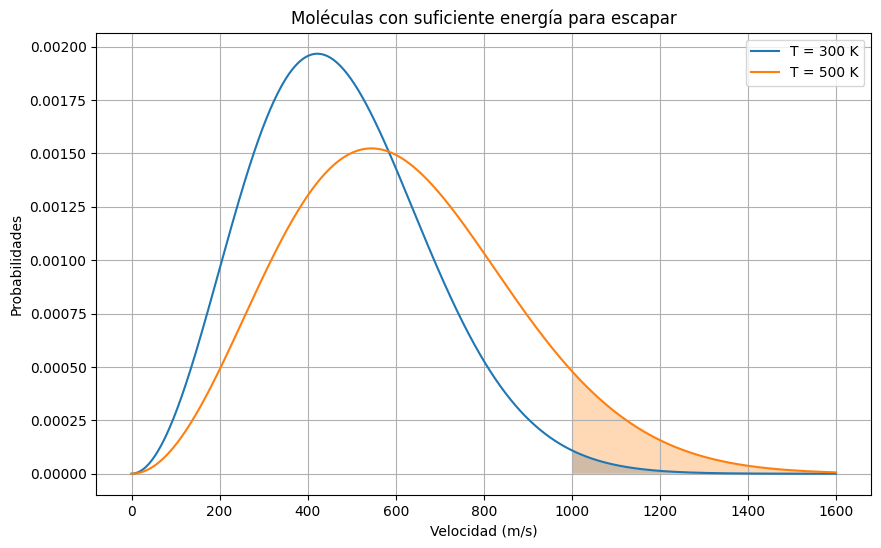
\includegraphics[width=0.9\textwidth]{./img/parte_2.png}
\end{figure}

\newpage
\begin{enumerate}
    % - Problema 1
    \vspace{\Pspace}
    \item ¿Qué ocurre con la forma de la distribución al aumentar la temperatura? \par
        % Respuesta:
        \vspace{\Aspace} \par
        { \color{azul}  
            Al aumentar la temperatura, la gráfica se hace más ancha y el punto más alto se mueve hacia velocidades mayores. 
            Esto significa que las moléculas se mueven más rápido.
        }

    % - Problema 2
    \vspace{\Pspace}
    \item ¿Qué sucede con el número de moléculas en la región v > v de escape? \par
        % Respuesta:
        \vspace{\Aspace} \par
        { \color{azul}  
            Cuando la temperatura aumenta, hay más moléculas con velocidades mayores a la velocidad de escape. 
            Esto pasa porque las moléculas tienen más energía.
        }

    % - Problema 3
    \vspace{\Pspace}
    \item Explica brevemente cómo esto se relaciona con la evaporación \par
        % Respuesta:
        \vspace{\Aspace} \par
        { \color{azul}  
            La evaporación pasa cuando algunas moléculas logran escapar del líquido. 
            Si la temperatura aumenta, más moléculas pueden escapar, por eso la evaporación ocurre más rápido.
        }
\end{enumerate}



\newpage
\Large{ \textbf{ Parte 3 } } \\
Completa el código para:
\begin{itemize}
    \item Calcular el área bajo la curva total
    \item Calcular el área para v > v de escape
    \item Obtener la fracción de moléculas que pueden evaporarse
\end{itemize}

\vspace{0.3cm}
\includesvg[height=0.8em]{./img/python_logo.svg} Python - Área total bajo la curva, área de alta velocidad y fracción de moléculas que escapan
\begin{lstlisting}
# Área total (debe ser ~1)
area_total = np.trapezoid(f1, v)

# Área de alta velocidad (evaporación)
area_escape = np.trapezoid(f1[v > v_escape], v[v > v_escape])

# Fracción de moléculas que escapan
fraccion = area_escape / area_total

print("Área total: ", area_total)
print("Área de escape: ", area_escape)
print("Fracción que puede evaporarse: ", fraccion)
\end{lstlisting}

\vspace{0.3cm}
\includesvg[height=0.7em]{./img/terminal_icon.svg} Output en terminal
\vspace{-0.5cm}
\begin{minted}{python}
    Área total:  0.9999974603866159
    Área de escape:  0.010450125807043768
    Fracción que puede evaporarse:  0.010450152346390533
\end{minted}

Comparar la fracción de moléculas que pueden evaporarse dependiendo de la temperatura del sistema. \par
\vspace{0.3cm}
\includesvg[height=0.8em]{./img/python_logo.svg} Python - Moléculas que pueden evaporarse / Temperatura del sistema
\begin{lstlisting}
area_escape_T1 = np.trapezoid(f1[v > v_escape], v[v > v_escape])
area_escape_T2 = np.trapezoid(f2[v > v_escape], v[v > v_escape])
print("Fracción T1: ", area_escape_T1)
print("Fracción T2: ", area_escape_T2)
\end{lstlisting}

\vspace{0.3cm}
\includesvg[height=0.7em]{./img/terminal_icon.svg} Output en terminal
\vspace{-0.5cm}
\begin{minted}{python}
    Fracción T1:  0.010450125807043768
    Fracción T2:  0.07969796311432695
\end{minted}

\newpage
\begin{enumerate}
    % - Problema 1
    \vspace{\Pspace}
    \item ¿Cuál temperatura tiene mayor área en la región de escape? \par
        % Respuesta:
        \vspace{\Aspace} \par
        { \color{azul}  
            La temperatura de 500 K tiene un área mayor en la región de escape. \
            Esto significa que hay más moléculas con suficiente velocidad para escapar.
        }

    % - Problema 2
    \vspace{\Pspace}
    \item ¿El cambio en el área es pequeño o grande? \par
        % Respuesta:
        \vspace{\Aspace} \par
        { \color{azul}  
            El cambio es grande, ya que la fracción pasa de aproximadamente 0.01 a casi 0.08. 
            Esto muestra que al aumentar la temperatura, muchas más moléculas pueden escapar.
        }

    % - Problema 3
    \vspace{\Pspace}
    \item ¿Por qué esto explica que la evaporación aumente rápidamente con la temperatura? \par
        % Respuesta:
        \vspace{\Aspace} \par
        { \color{azul}  
            Esto explica que la evaporación aumente porque al subir la temperatura, 
            más moléculas tienen la energía necesaria para escapar del líquido. 
            Por eso la evaporación ocurre mucho más rápido.
        }
\end{enumerate}
\end{document}
